\documentclass{article}

\usepackage{amsmath}
\usepackage{pgfplots}

\pgfplotsset{compat=1.18}

\begin{document}
\begin{enumerate}
	\item \begin{enumerate}
		      \item
		            \begin{flalign*}
			             & L(x) = f(0) + f'(0)(x - 0)                      & \\
			             & L(x) = 1 + 3(1 - x)^2 (-1) x = 1 - 3(1 - x)^2 x & \\
			             & L(x) = 1 + 3(1 - x)^2 (-1) x = 1 - 3x           & \\
		            \end{flalign*}

		      \item
		            \begin{flalign*}
			             & L(x) = f(e^2) + f'(e^2)(x - e^2)                                                     & \\
			             &                                                                                      & \\
			             & f'(k) = \frac{ d }{ dx } \left( \frac{ k^2 }{ \ln k } \right)                        & \\
			             & f'(k) = \frac{ (k^2)' \ln k - k^2 (\ln k)' }{ (\ln k)^2 }                            & \\
			             & f'(k) = \frac{ 2k \ln k - k^2 \frac{ 1 }{ k } }{ (\ln k)^2 }                         & \\
			             & f'(k) = \frac{ 2k \ln k - k }{ (\ln k)^2 }                                           & \\
			             &                                                                                      & \\
			             & L(k) = \frac{ e^4 }{ \ln e^2 } + \frac{ 2e^2 \ln e^2 - e^2 }{ (\ln e^2)^2 }(k - e^2) & \\
			             & L(k) = \frac{ e^4 }{ 2 } + \frac{ 3e^2 }{ 4 } (k - e^2)                              & \\
		            \end{flalign*}
	      \end{enumerate}

	\item \begin{flalign*}
		       & \lim_{x \to 2} \frac{ f(x) - 5 }{ x - 2 } = 10 & \\
	      \end{flalign*}

	\item \begin{flalign*}
		       & y' = 3x^2 + 3                         & \\
		       & 3x^2 + 3 = 6                          & \\
		       & x = \pm 1                             & \\
		       & ((1, 4), (-1, -4))                    & \\
		       & 4 = 6 \times 1 + c \implies x = -2    & \\
		       & -4 = 6 \times (-1) + c \implies x = 2 & \\
		       & y_1 = 6x + 2                          & \\
		       & y_2 = 6x - 2                          & \\
	      \end{flalign*}

	\item
	\item
	\item
	\item
	      \begin{flalign*}
		       & C/h = kv^3 \implies C = k h v^3                                               & \\
		       & h = \frac{ S }{ v }                                                           & \\
		       & h = \frac{ S }{ v - a }                                                       & \\
		       & C = k \frac{ S v^3 }{ v - a }                                                 & \\
		       & T(v) = \frac{ kS v^3 }{ v - a }                                               & \\
		       & T'(v) = kS \left[\frac{ d }{ dx } \left( \frac{ v^3 }{ v - a } \right)\right] & \\
		       & T'(v) = kS \left( \frac{ 3v^2 (v - a) - v^3 }{ (v - a)^2 } \right)            & \\
		       & T'(v) = kS \left( \frac{ 3v^3 - 3av^2 - v^3 }{ (v - a)^2 } \right)            & \\
		       & T'(v) = kS \left( \frac{ 2v^3 - 3av^2 }{ (v - a)^2 } \right)                  & \\
		       & \frac{ 2v^3 - 3av^2 }{ (v - a)^2 } = 0                                        & \\
		       & 2v^3 - 3av^2 = 0                                                              & \\
		       & 2v - 3a = 0 \implies v = \frac{ 3 }{ 2 } a                                    & \\
	      \end{flalign*}

	\item
	\item \begin{flalign*}
		       & Cu_a(m) = 5m                                                      & \\
		       & Cu_l(m) = 3m                                                      & \\
		       & h = 100                                                           & \\
		       & \sqrt{b^2 + h^2} = 1000                                           & \\
		       & b^2 = 1000^2 - 100^2 = (1000 + 100)(1000 - 100) = 1100 \times 900 & \\
		       & = 11 \times 9 \times 100^2                                        & \\
		       & b = \sqrt{11} \times 3 \times 100 = 300 \sqrt{11}                 & \\
		       & Cu_t(t_1, a, t_2) = Cu_l(t_1) + Cu_a(a) + Cu_l(t_2)               & \\
		       & Cu_t(t_1, a, t_2) = 3t_1 + 5a + 3t_2                              & \\
	      \end{flalign*}

	\item \begin{enumerate}
		      \item \begin{flalign*}
			             & w + 2 \ge 0 \implies w \ge -2 & \\
			             & D(f) = [-2, + \infty)         & \\
		            \end{flalign*}

		      \item \begin{flalign*}
			             & w^2 - \ln(w + 2) = 0 & \\
		            \end{flalign*}
		      \item \leavevmode\vadjust{\vspace{-\baselineskip}}\newline
		            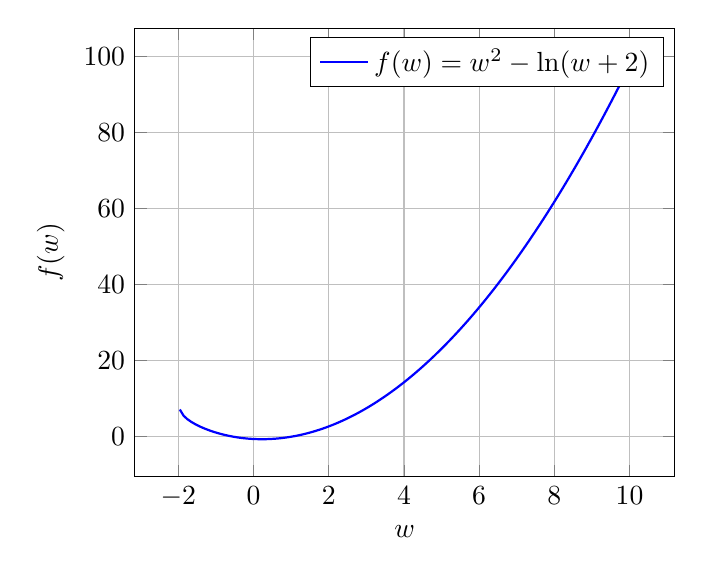
\begin{tikzpicture}
			            \begin{axis}[
					            xlabel=$w$,
					            ylabel=$f(w)$,
					            grid=both,
				            ]

				            \addplot[domain=-10:10, samples=200, thick, blue] {x^2 - ln(x + 2)};
				            \addlegendentry{$f(w) = w^2 - \ln(w + 2)$}
			            \end{axis}
		            \end{tikzpicture}
	      \end{enumerate}

	\item \begin{enumerate}
		      \item Certamente, uma função contínua em um intervalo fechado
		            \([a, b]\) pode existir sem apresentar pontos críticos em seu
		            interior. \\

		            Um exemplo simples seria uma função constante dentro do
		            intervalo \([a, b]\). Se considerarmos uma função \(f(x)\)
		            constante nesse intervalo, não haverá variação na função
		            dentro do intervalo, e, portanto, não existirão pontos
		            críticos, pois não há mudança na inclinação ou na
		            concavidade. \\

		            Portanto, uma função constante em um intervalo fechado
		            \([a, b]\) é contínua em todo o intervalo, mas não tem
		            pontos críticos, já que não há mudança na função ao longo
		            desse intervalo. \\

		      \item
		            Uma função contínua em um intervalo fechado \([a, b]\)
		            pode, sim, existir sem apresentar pontos críticos em seu
		            interior. \\

		            Um exemplo clássico é uma função constante no intervalo
		            \([a, b]\). Se considerarmos uma função \(f(x)\) constante
		            nesse intervalo, não haverá variação na função dentro do
		            intervalo, e, portanto, não existirão pontos críticos, já
		            que não há mudança na inclinação ou concavidade. \\

		            Portanto, uma função constante em um intervalo fechado
		            \([a, b]\) é contínua em todo o intervalo, mas não tem
		            pontos críticos, pois não há mudança na função ao longo
		            desse intervalo. \\

		      \item
		            Não é verdade que uma função contínua em \([a, b]\) com um
		            mínimo local em \(c \in (a, b)\) necessariamente tenha
		            pontos críticos no intervalo \((a, b)\). Além disso, a
		            existência da derivada não é uma exigência para a presença
		            de um mínimo local em \(x = c\). \\

		            Um exemplo disso é uma função com um mínimo local em \(c\)
		            mas sem pontos críticos. Por exemplo, a função \(f(x) =
		            |x|\) possui um mínimo local em \(x = 0\), mas não possui
		            pontos críticos no intervalo \((-1, 1)\) porque a derivada
		            não existe em \(x = 0\). \\

		            Portanto, a presença de um mínimo local em \(c\) não
		            implica que a função tenha pontos críticos no intervalo
		            \((a, b)\), e a derivada não precisa existir em \(x = c\)
		            para que haja um mínimo local nesse ponto. \\

		      \item
		            Sim, é possível ter uma função contínua em um intervalo fechado \([a, b]\) que
		            possui um máximo absoluto em \(x = a\) e um mínimo absoluto em \(x
		            = b\). Isso ocorre quando a função é constante nesse intervalo. \\

		            Se considerarmos uma função \(f(x)\) que é constante em
		            \([a, b]\) e diferente de constantes em \(x = a\) e \(x =
		            b\), teremos um exemplo de uma função que alcança seu valor
		            máximo absoluto em \(x = a\) e seu valor mínimo absoluto em
		            \(x = b\). \\

		      \item
		            Sim, uma função que atenda a essas condições seria uma função constante no
		            intervalo \([a, b]\). Se \(f(x)\) é uma função constante nesse intervalo, a
		            derivada \(f'(x)\) seria zero para qualquer \(x\) no intervalo \((a, b)\). \\

		            Se considerarmos \(f(x) = c\) para \(x \in [a, b]\), onde \(c\) é uma
		            constante, a derivada \(f'(x)\) será zero, pois a derivada de uma constante é
		            zero. Nesse caso, a função terá um mínimo absoluto em \(x = a\) e um máximo
		            absoluto em \(x = b\) sem ter pontos críticos no intervalo \((a, b)\). \\

		            Portanto, a função constante \(f(x) = c\) para \(x \in [a, b]\) é um exemplo de
		            uma função que atende às condições especificadas: mínimo absoluto em \(x = a\),
		            máximo absoluto em \(x = b\) e \(f'(x) = 0\) para qualquer \(x\) no intervalo
		            \((a, b)\). \\

		      \item
		            Uma função contínua em um intervalo fechado \([a, b]\) com um mínimo absoluto
		            em \(x_1\) e um máximo absoluto em \(x_2\) onde \(x_1 = x_2\) não é possível,
		            exceto em um caso particular. \\

		            Em um cenário onde \(x_1 = x_2\) no intervalo \([a, b]\), a função deveria ter
		            ambos os extremos do intervalo como mínimo e máximo absolutos, o que só é
		            possível se a função for constante nesse intervalo, ou seja, se \(f(x)\) for
		            uma constante em \([a, b]\). \\

		            Assim, a única situação na qual uma função contínua em um intervalo \([a, b]\)
		            poderia ter um mínimo absoluto em \(x_1\) e um máximo absoluto em \(x_2\) com
		            \(x_1 = x_2\) seria se a função fosse uma constante nesse intervalo. \\

		            Portanto, a resposta seria que somente uma função constante em todo o intervalo
		            \([a, b]\) teria mínimo e máximo absolutos no mesmo ponto, se \(x_1 = x_2\). \\

		      \item Sim. Uma função que quebrasse esta regra violaria o teste de derivada. \\

		      \item
		            Sim, é possível ter uma função derivável \(f(x)\) no intervalo aberto \((a,
		            b)\) sem possuir pontos extremos nesse intervalo. \\

		            Um exemplo seria a função \(f(x) = x\) no intervalo aberto \((a, b)\). Essa
		            função é derivável em todos os pontos do intervalo aberto, porém não possui um
		            máximo ou mínimo local nesse intervalo. Como é uma função linear e não tem
		            pontos de inflexão, ela não possui pontos extremos. \\

		            Portanto, é possível ter funções deriváveis no intervalo aberto \((a, b)\) sem
		            apresentar pontos extremos nesse intervalo. \\
	      \end{enumerate}
\end{enumerate}
\end{document}
